\documentclass[xelatex,10pt]{beamer}
\usetheme{metropolis}

\usepackage[english]{babel}
\usepackage{graphicx}
\usepackage{textpos}
\usepackage{xcolor}
\definecolor{mauve}{rgb}{0.86, 0.82, 1.0}
\definecolor{dkgreen}{rgb}{0,0.6,0}
\usepackage{pgfpages}
\usepackage{listings}

\setsansfont[BoldFont={OpenSans-Bold}]{Fira Sans}

\lstdefinelanguage{d}{
	morekeywords={abstract,alias,align,asm,assert,auto,body,bool,break,byte,
		case,cast,catch,cdouble,cent,cfloat,char,class,const,continue,creal,
		dchar,debug,default,delegate,delete,deprecated,do,double,else,enum,
		export,extern,false,final,finally,float,for,foreach,foreach_reverse,
		function,goto,idouble,if,ifloat,immutable,import,in,inout,int,
		interface,invariant,ireal,is,lazy,long,macro,mixin,module,new,nothrow,
		null,out,override,package,pragma,private,protected,public,pure,real,
		ref,return,scope,shared,short,static,struct,string,wstring,dstring,
		super,switch,synchronized,template,this,throw,true,try,typedef,typeid,
		typeof,ubyte,ucent,uint,ulong,union,unittest,ushort,version,void,
		volatile,wchar,while,with,size_t,hash_t,__traits
	},
	sensitive=True,
	morecomment=[l]{//},
	morecomment=[s]{/\*}{\*/},
	morestring=[b]"
}
\lstdefinelanguage{typescript}{
	morekeywords={abstract,alias,align,asm,assert,auto,body,bool,break,byte,
		case,cast,catch,cdouble,cent,cfloat,char,class,const,continue,creal,
		dchar,debug,default,delegate,delete,deprecated,do,double,else,enum,
		export,extern,false,final,finally,float,for,foreach,foreach_reverse,
		function,goto,idouble,if,ifloat,immutable,import,in,inout,int,
		interface,invariant,ireal,is,lazy,long,macro,mixin,module,new,nothrow,
		null,out,override,package,pragma,private,protected,public,pure,real,
		ref,return,scope,shared,short,static,struct,string,wstring,dstring,
		super,switch,synchronized,template,this,throw,true,try,typedef,typeid,
		typeof,ubyte,ucent,uint,ulong,union,unittest,ushort,version,void,
		volatile,wchar,while,with,size_t,hash_t,number,extends,constructor
	},
	sensitive=True,
	morecomment=[l]{//},
	morecomment=[s]{/\*}{\*/},
	morestring=[b]",
	morestring=[b]'
}


\lstset{
	language=d,
	basicstyle=\footnotesize\ttfamily, % Standardschrift
	numbers=left,               % Ort der Zeilennummern
	numberstyle=\tiny,          % Stil der Zeilennummern
	%stepnumber=2,               % Abstand zwischen den Zeilennummern
	captionpos=b,
	numbersep=5pt,              % Abstand der Nummern zum Text
	tabsize=4,                  % Groesse von Tabs
	extendedchars=true,         %
	breaklines=true,            % Zeilen werden Umgebrochen
	showspaces=false,           % Leerzeichen anzeigen ?
	showtabs=false,             % Tabs anzeigen ?
	%frame=b,
	rulecolor=\color[cmyk]{0.0, 0.0, 0.0, 0.316},
	xleftmargin=17pt,
	%xleftmargin=0pt,
	framexleftmargin=17pt,
	framexrightmargin=5pt,
	framexbottommargin=4pt,
	keywordstyle=\color{blue},          % keyword style
	commentstyle=\color{dkgreen},       % comment style
	stringstyle=\color{red},         % string literal style
	showstringspaces=false,    % Leerzeichen in Strings anzeigen ?        
	escapeinside={/+}{+/},
	title=\lstname,
    postbreak=\raisebox{0ex}[0ex][0ex]{\ensuremath{\color{red}\hookrightarrow\space}}
}

%\setbeamertemplate{note page}{\pagecolor{yellow!5}\insertnote}\usepackage{palatino}
%\setbeameroption{show notes on second screen}

\beamertemplatenavigationsymbolsempty

\usepackage{xkeyval}
%\presetkeys{todonotes}{inline}{}
\usepackage[disable]{todonotes}

\title{An Introduction to D and the Degenerator}
\author{Robert "burner" Schadek}
\date{Jan 10, 2017}

\begin{document}
\maketitle

\section{Make C++ Great Again}
\begin{frame}{Procedural}
\lstinputlisting[basicstyle=\footnotesize,caption={},linerange=13-24,
	firstnumber=1,numbers=none,xleftmargin=-5mm
]{fun_with_d.d}
\end{frame}

\begin{frame}{Object Oriented 1/2}
\begin{columns}[T]
\begin{column}{0.49\linewidth}
\lstinputlisting[basicstyle=\footnotesize,caption={},linerange=94-108,
	firstnumber=1,numbers=none,xleftmargin=-5mm
]{fun_with_d.d}
\end{column}
\begin{column}{0.50\linewidth}
\lstinputlisting[basicstyle=\footnotesize,caption={},linerange=120-126,
	firstnumber=1,numbers=none,xleftmargin=-1mm
]{fun_with_d.d}
\end{column}
\end{columns}
\end{frame}

\begin{frame}{Object Oriented 2/2}
\lstinputlisting[basicstyle=\footnotesize,caption={},linerange=110-118,
	firstnumber=1,numbers=none,xleftmargin=-5mm
]{fun_with_d.d}
\lstinputlisting[basicstyle=\footnotesize,caption={},linerange=128-131,
	firstnumber=1,numbers=none,xleftmargin=-5mm
]{fun_with_d.d}
\end{frame}

\begin{frame}{Templates 1/3}
\lstinputlisting[basicstyle=\footnotesize,caption={},linerange=41-55,
	firstnumber=1,numbers=none,xleftmargin=-5mm
]{fun_with_d.d}
\end{frame}

\begin{frame}{Templates 2/3}
\lstinputlisting[basicstyle=\footnotesize,caption={},linerange=61-67,
	firstnumber=1,numbers=none,xleftmargin=-5mm
]{fun_with_d.d}
\end{frame}

\begin{frame}{Templates 3/3}
\lstinputlisting[basicstyle=\footnotesize,caption={},linerange=69-78,
	firstnumber=1,numbers=none,xleftmargin=-5mm
]{fun_with_d.d}
\end{frame}

\begin{frame}{Compile Time Function Execution (CTFE)}
\lstinputlisting[basicstyle=\footnotesize,caption={},linerange=153-166,
	firstnumber=1,numbers=none,xleftmargin=-5mm
]{fun_with_d.d}
\end{frame}

\subsection{Functional}
\begin{frame}{Functional}
\lstinputlisting[basicstyle=\footnotesize,caption={},linerange=186-200,
	firstnumber=1,numbers=none,xleftmargin=-5mm
]{fun_with_d.d}
\end{frame}

\begin{frame}{Pure Fun(ctions)}
\lstinputlisting[basicstyle=\footnotesize,caption={},linerange=214-226,
	firstnumber=1,numbers=none,xleftmargin=-5mm
]{fun_with_d.d}
\end{frame}

\begin{frame}{Static Introspection 1/2}
\lstinputlisting[basicstyle=\footnotesize,caption={},linerange=260-264,
	firstnumber=1,numbers=none,xleftmargin=-5mm
]{fun_with_d.d}

\lstinputlisting[basicstyle=\footnotesize,caption={},linerange=283-288,
	firstnumber=1,numbers=none,xleftmargin=-5mm
]{fun_with_d.d}
\end{frame}

\begin{frame}{Static Introspection 1/2}
\lstinputlisting[basicstyle=\footnotesize,caption={},linerange=266-281,
	firstnumber=1,numbers=none,xleftmargin=-8mm
]{fun_with_d.d}
\end{frame}

\begin{frame}{tl;dr}
\begin{itemize}
	\item Template \lstinline@struct@es/\lstinline@class@es
	\item User Defined Attributes \lstinline@\@Bar("Whatever")@
	\item \lstinline@foreach@ and Ranges
	\item \lstinline@module@s
	\item Compiler dmd, gdc and ldc
	\item C ABI, C++ ABI compatibility
\end{itemize}
\end{frame}

\section{Degenerator}
\begin{frame}
	\frametitle{Everything is wrong}
	\begin{itemize}
		\onslide<1->{\item Waterfall Model} \onslide<2->{\(\leftarrow\) 
			no change, never}
		\onslide<7->{\item UML} \onslide<8->{\(\leftarrow\) just kill me
			already}

		\item[] { \onslide<1-8>{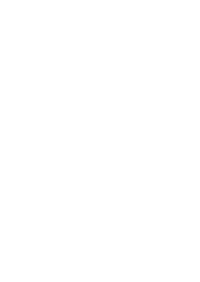
\includegraphics[width=0.2\textwidth]{Stick1.png}}
			\only<9>{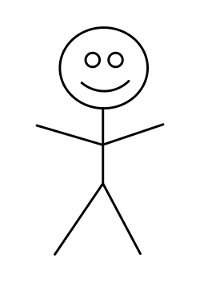
\includegraphics[width=0.2\textwidth]{Stick.png}}
			\only<10>{\hspace{-1.31mm}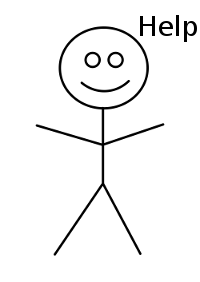
\includegraphics[width=0.2\textwidth]
				{Stick2.png}}
		}

		\onslide<5->{\item Agile Methods} \onslide<6->{\(\leftarrow\) just
			hacking, with fancy names}
		\onslide<3->{\item Hacking} \onslide<4->{\(\leftarrow\) no plan
			to speak of, just change}
		
	\end{itemize}
	
\end{frame}

\begin{frame}
	\frametitle{What do we want}
	\begin{itemize}
		\item Speak about the system at different levels of detail
		with different people
		\item Quickly introduce people to the system
		\item Keep classes (Model) synchronized across
		\begin{itemize}
			\item Frontend
			\item Server
			\item \(\dots\)
		\end{itemize}
		\item Write only one model for everything, to keep stuff DRY
		\item Have a line based description, because git
		\item Generate everything possible from the Model, to keep Model and
Source in sync
	\end{itemize}
\end{frame}

\section{Introducing the C4 Architecture}
\begin{frame}[plain]
\begin{textblock*}{0cm}(-1cm,-4.7cm)
	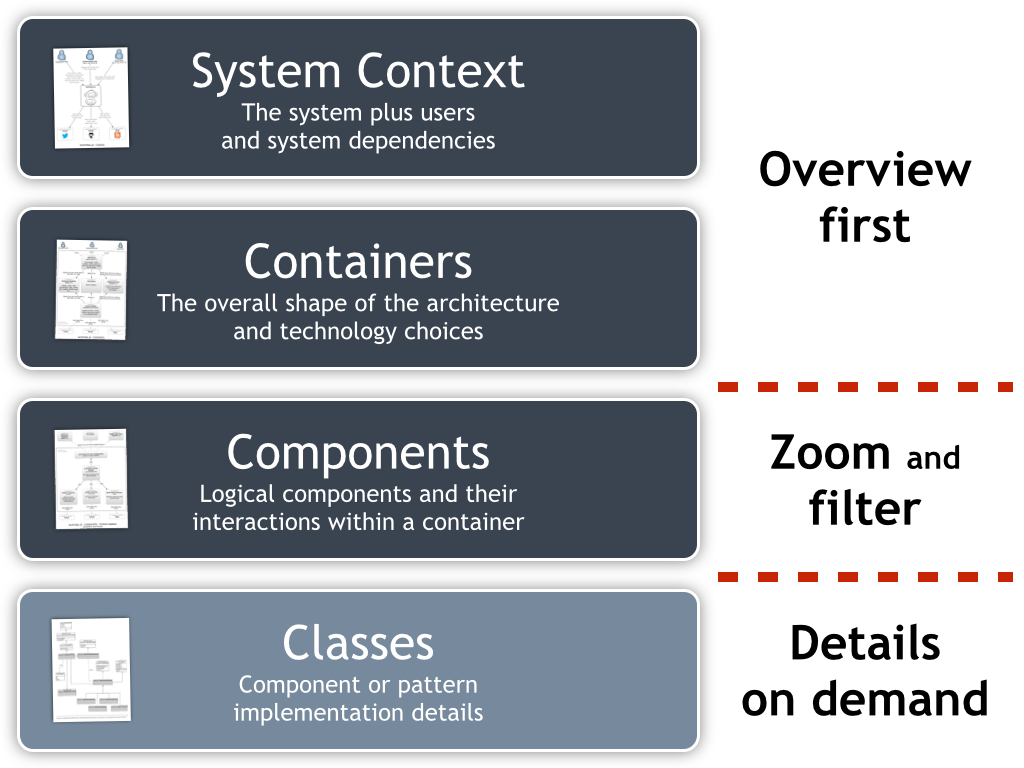
\includegraphics[width=1.0\paperwidth]{c4overview.png}
\end{textblock*}
\end{frame}
\begin{frame}[plain]
\begin{textblock*}{0cm}(-1cm,-4.7cm)
	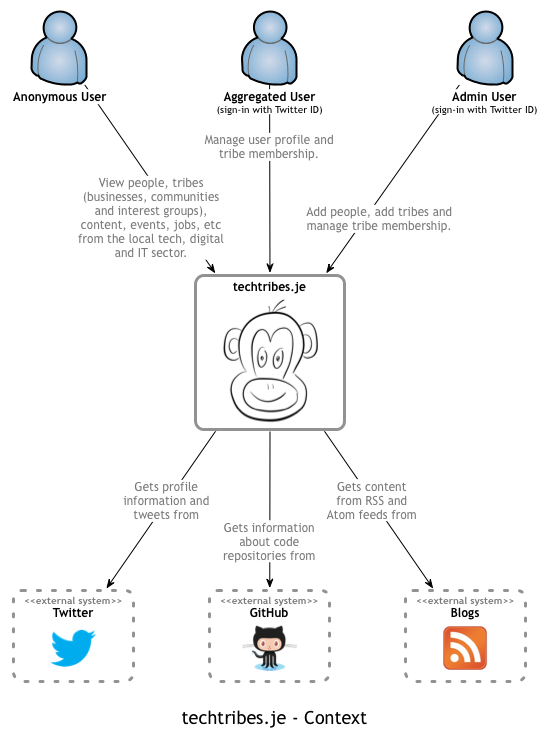
\includegraphics[width=1.0\paperwidth]{c4systemcontext.png}
\end{textblock*}
\end{frame}
\begin{frame}[plain]
\begin{textblock*}{0cm}(-1cm,-11.7cm)
	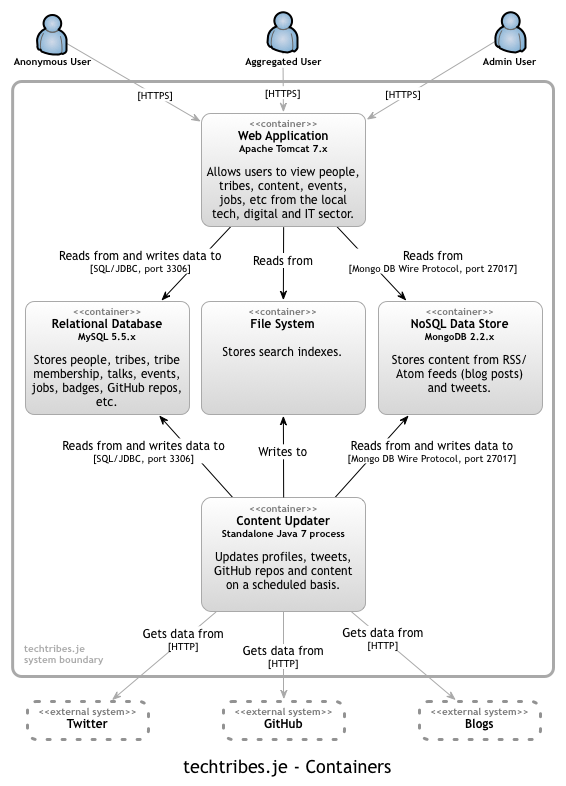
\includegraphics[width=1.0\paperwidth]{c4container.png}
\end{textblock*}
\end{frame}
\begin{frame}[plain]
\begin{textblock*}{0cm}(-1cm,-4.7cm)
	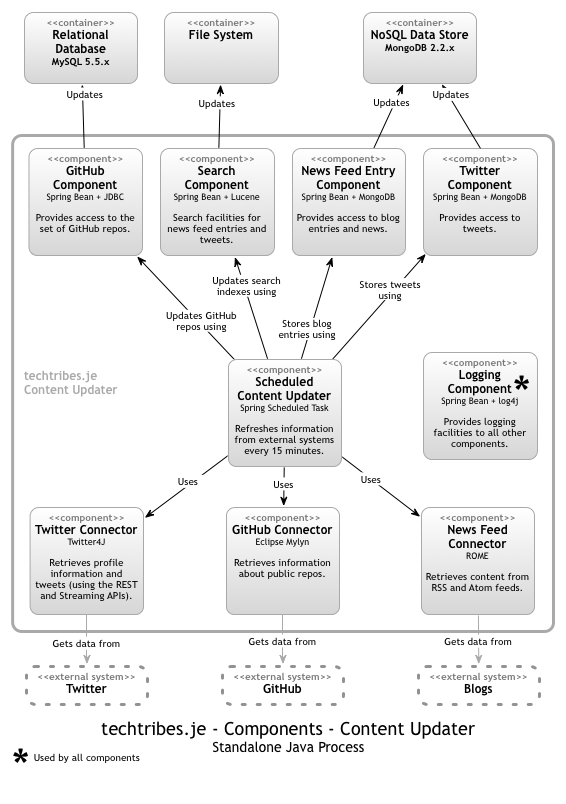
\includegraphics[width=1.0\paperwidth]{c4components.png}
\end{textblock*}
\end{frame}

\begin{frame}
	\frametitle{Structurizr}
	\begin{itemize}
		\item Implements C4 Architecture Model 
		\item Java library to build the model
			\pause
		\begin{itemize}
			\item Its code, its fits into git
		\end{itemize}
			\pause
		\item Structurizr generates code
			\pause
		\item Only Java and .net
	\end{itemize}
\end{frame}
\begin{frame}[plain]
\begin{textblock*}{0cm}(-1cm,-4.4cm)
	
\includegraphics[width=1.0\paperwidth]{picardwtf.jpg}
\end{textblock*}
\end{frame}

\section{How hard can it be}
\begin{frame}
	\frametitle{How do we approach the development}
	\begin{itemize}
		\item We're not gonne create a new language\pause, at first\pause,
			most likely
			\pause
		\item The model (ast) is pretty simple
			\pause
		\begin{itemize}
			\item The world
			\item The world has
			\item Actors, software/hardware systems
			\item A software systems has
			\item Containers (everything with a unique pid)
			\item A container has
			\item Components (think \lstinline@module@) and classes
			\item A component has
			\item Components and classes
			\item Classes have members
				\pause
			\item Connections between the above
			\begin{itemize}
				\item UML Association, Aggregation, Composition, Dependency, \(\dots\)
			\end{itemize}
			\item Additional informations, names, descriptions
		\end{itemize}
	\end{itemize}
\end{frame}

\begin{frame}
	\frametitle{Using Degenerator 1/2}
	\lstinputlisting[basicstyle=\footnotesize,caption={},linerange=10-15,
		firstnumber=10,numbers=none,xleftmargin=-1cm
	]{Sources/app.d}
	\pause
	\lstinputlisting[basicstyle=\footnotesize,caption={},linerange=17-19,
		firstnumber=17,numbers=none,xleftmargin=-1cm
	]{Sources/app.d}
\end{frame}
\begin{frame}
	\frametitle{Using Degenerator 2/4}
	\lstinputlisting[basicstyle=\footnotesize,caption={},linerange=45-49,
		firstnumber=45,numbers=none,xleftmargin=-1cm
	]{Sources/app.d}
	\pause
	\lstinputlisting[basicstyle=\footnotesize,caption={},linerange=61-63,
		firstnumber=61,numbers=none,xleftmargin=-1cm
	]{Sources/app.d}
\end{frame}

\begin{frame}
	\frametitle{Using Degenerator 3/4}
	\lstinputlisting[basicstyle=\small,caption={},linerange=61-63,
		firstnumber=61,numbers=none,xleftmargin=-1cm
	]{Sources/app.d}
	\pause
	\lstinputlisting[basicstyle=\small,caption={},linerange=68-71,
		firstnumber=68,numbers=none,xleftmargin=-1cm
	]{Sources/app.d}
\end{frame}
\begin{frame}
	\frametitle{Using Degenerator 4/4}
	\lstinputlisting[basicstyle=\small,caption={},linerange=77-79,
		firstnumber=77,numbers=none,xleftmargin=-1cm
	]{Sources/app.d}
	\pause
	\lstinputlisting[basicstyle=\small,caption={},linerange=90-92,
		firstnumber=90,numbers=none,xleftmargin=-1cm
	]{Sources/app.d}
\end{frame}

\begin{frame}[fragile]
	\frametitle{Types in Degenerator}
	\begin{itemize}
		\item Types \pause e.g. strings are not always strings
		\pause
		\begin{itemize}
			\item D string
			\item MySQL text
			\item C++ std::string
		\end{itemize}
	\end{itemize}
	\pause
	\begin{lstlisting}[basicstyle=\small,xleftmargin=0.2cm,numbers=none]
struct Type {
    string name;
    string[string] typeMapping;
}

auto pwdHash = Type("PasswordString"); /+\pause+/
pwdHash.typeMappings["D"] = "string";
pwdHash.typeMappings["MySQL"] = "VARCHAR(128)";
\end{lstlisting}
	\vspace{-1cm}
%\begin{itemize}
%	\item Similar types with different behaviour across containers
%\end{itemize}
\end{frame}

\begin{frame}
	\frametitle{Generating}
	\lstinputlisting[basicstyle=\small,caption={},linerange=106-110,
		firstnumber=106,numbers=none,xleftmargin=-1.1cm
	]{Sources/app.d}
\end{frame}

\begin{frame}
	\frametitle{The World}
	\begin{textblock*}{0cm}(-1.2cm,-2.0cm)
		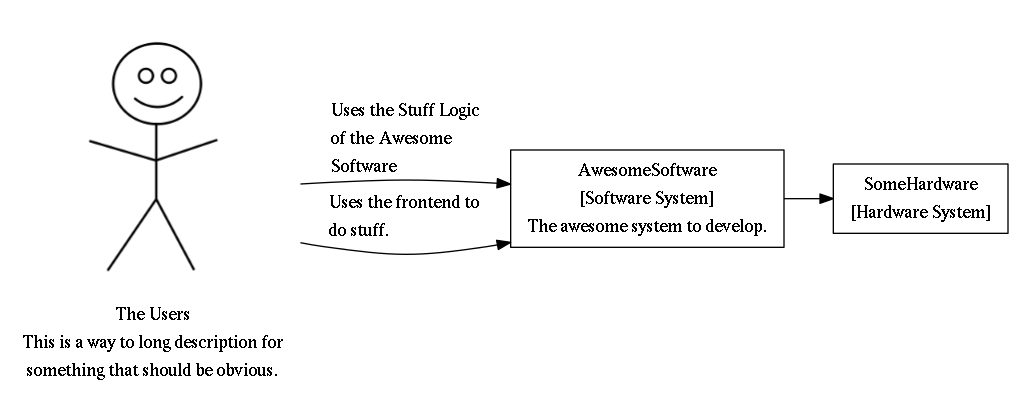
\includegraphics[width=1.0\paperwidth]{theworld.png}
	\end{textblock*}
\end{frame}

\begin{frame}
	\frametitle{The World and Containers}
	\begin{textblock*}{0cm}(-1.2cm,-2.0cm)
		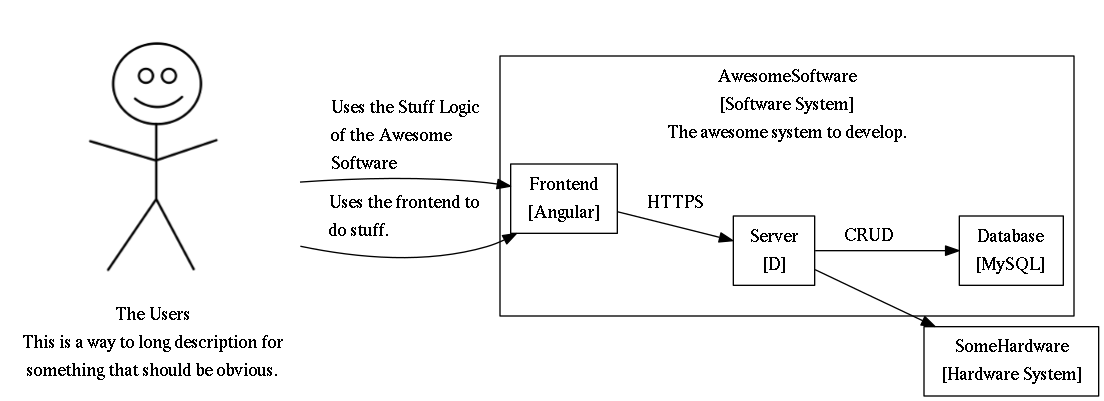
\includegraphics[width=1.0\paperwidth]{theworldandcontainer.png}
	\end{textblock*}
\end{frame}

%\begin{frame}
%	\frametitle{Actors, Containers and Components}
%	\begin{textblock*}{0cm}(-1.2cm,-2.0cm)
%		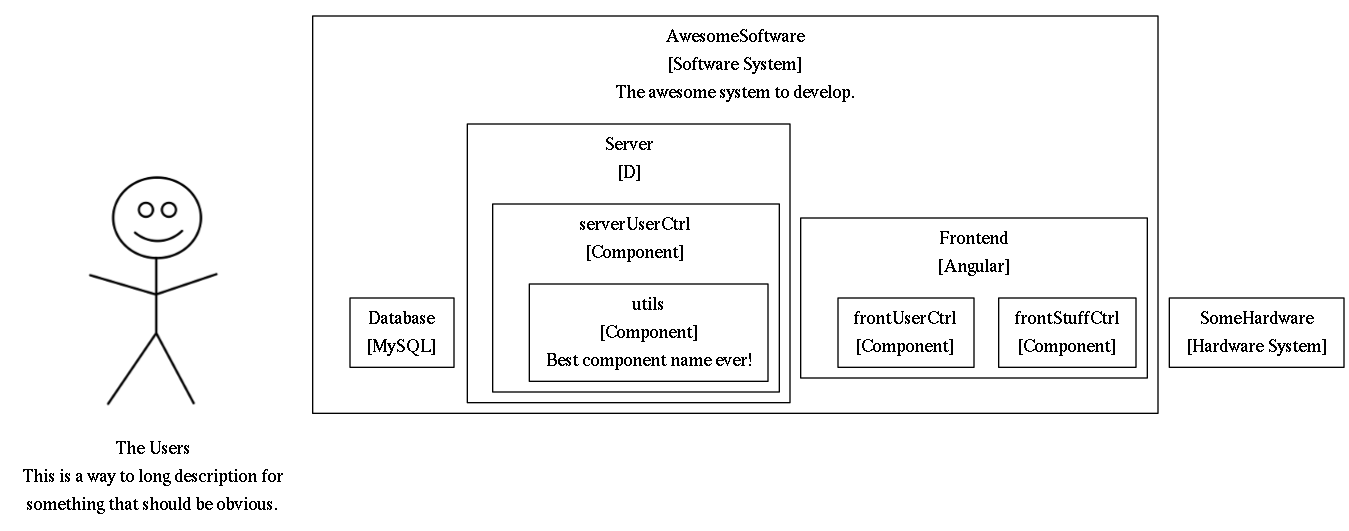
\includegraphics[width=1.0\paperwidth]{theworldcontainercomponents.png}
%	\end{textblock*}
%\end{frame}

\begin{frame}
	\frametitle{Awesome Software System}
	\begin{textblock*}{0cm}(-1.0cm,-4.0cm)
		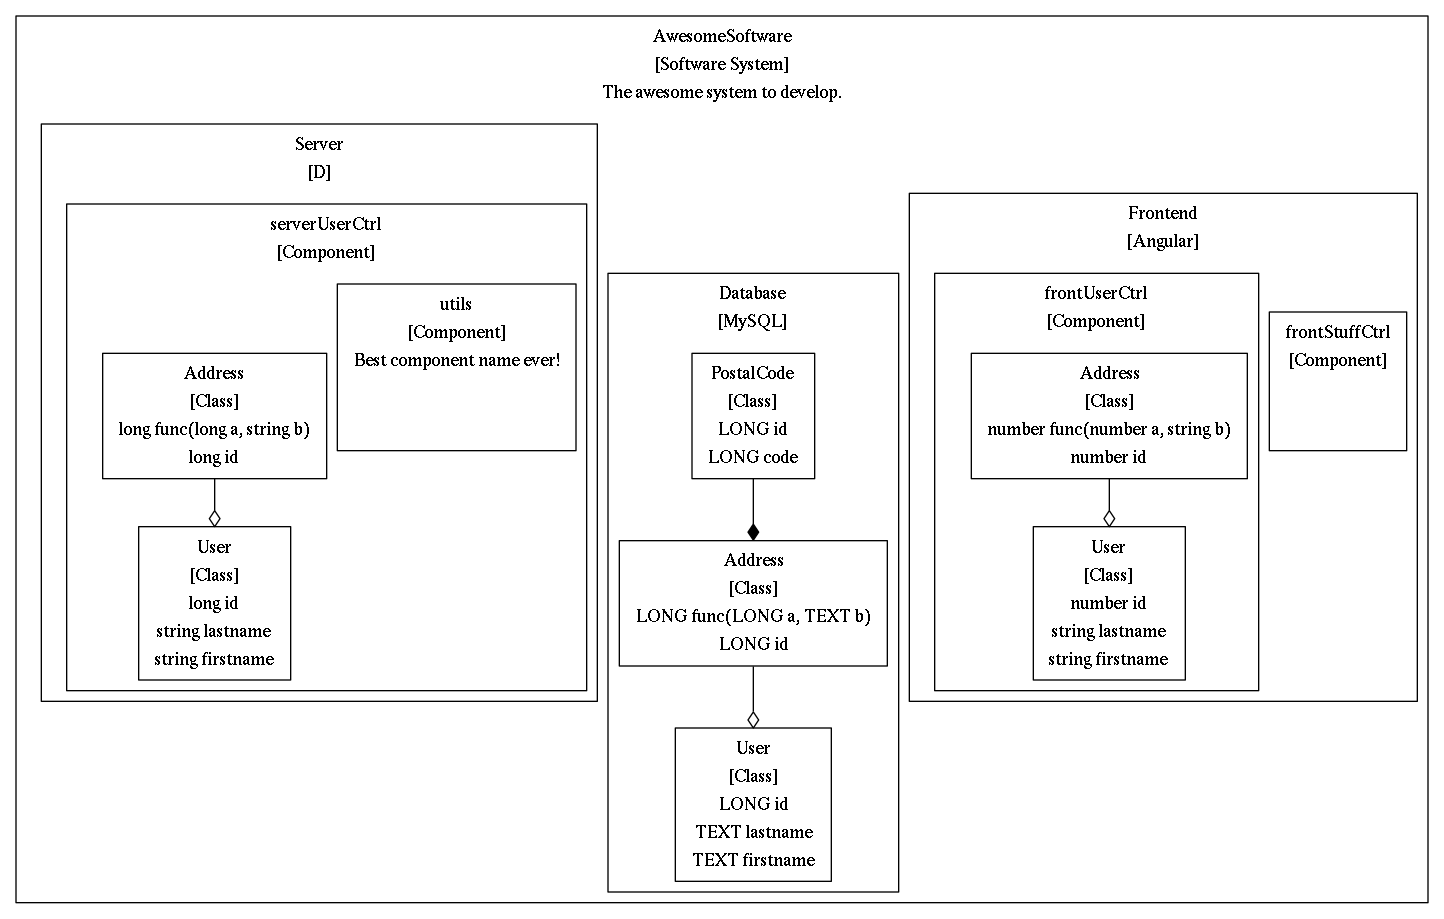
\includegraphics[width=1.0\paperwidth]{AwesomeSoftware.png}
	\end{textblock*}
\end{frame}

\begin{frame}
	\frametitle{Generating the Database CREATE TABLE Statements}
\begin{columns}[T]
\begin{column}{0.49\linewidth}
	\lstinputlisting[basicstyle=\scriptsize,language=SQL,caption={},
			numbers=none,xleftmargin=-0.5cm]
	{Sources/Address.sql}
	\vspace{12mm}
	\lstinputlisting[basicstyle=\scriptsize,language=SQL,caption={},numbers=none
		,xleftmargin=-0.5cm]
	{Sources/Address_User.sql}
\end{column}
\begin{column}{0.49\linewidth}
	\lstinputlisting[basicstyle=\scriptsize,language=SQL,caption={},numbers=none
		,xleftmargin=-0.4cm]
	{Sources/User.sql}
	\lstinputlisting[basicstyle=\scriptsize,language=SQL,caption={},numbers=none
			,xleftmargin=-0.4cm]
	{Sources/PostelCode.sql}
\end{column}
		
\end{columns}
\end{frame}

\begin{frame}
	\frametitle{What can we generate}
	\begin{itemize}
		\item Diagrams describing the project at different levels of detail
		\item Database schema
		\item phpmyadmin clones
		\item Database access code
		\item Data objects (D struct/class, Typescript interface/class, \(\dots\)
		\item Server skeletons
		\item Frontend skeletons
			\pause
		\item Graphviz mostly done, MySQL is getting there, Vibe.d and
			Angular2 next
	\end{itemize}
\end{frame}

\begin{frame}[plain]
\begin{textblock*}{0cm}(-1cm,-4.2cm)
	
\includegraphics[width=1.0\paperwidth]{picardpuppy.png}
	\todo{http://gryphon-shifter.deviantart.com/art/Captain-Picard-and-Puppies-458352865}
\end{textblock*}
\end{frame}

\begin{frame}
	\frametitle{The End}
	\begin{itemize}
		\item vibe.d \url{https://vibed.org}
		\item typescript \url{https://www.typescriptlang.org/}
		\item dstructtotypescript
			\url{https://github.com/burner/dstructtotypescript}
		\item C4 Architecture (Simon Brown) \url{http://www.codingthearchitecture.com}
		\item Structurizr \url{https://structurizr.com/}
		\item Degenerator \url{https://github.com/burner/Degenerator}
	\end{itemize}
\end{frame}

\end{document}
